\section{Flat pins across a long annulus}\label{sec:annuli}

The comparison in Theorem~\ref{sectors:positive-radius} concerns holes of
fixed positive radius. To connect such a hole to a microscopic source,
we need a pin-probability estimate on a long annulus: making the heights
equal on a middle band changes the probability that the heights are
equal at a distant end by a factor tending to one in the mesh limit
as the logarithmic annular length grows. Each of these events leaves
its common height free. We derive this estimate from
the absolute-pin input in Theorem~\ref{heights:pin-input}.

\subsection{Polygonal annuli and their bands}

Fix a small \(\varepsilon>0\), and choose a closed rectilinear polygon
\(P\), homeomorphic to a closed disk, with dyadic vertices and
\[
 B(0,1-\varepsilon)\subset P\subset B(0,1+\varepsilon).
\]
One may use a sufficiently fine staircase approximation to the circle,
chosen symmetrically in the four quadrants. All side lengths and
passages in the resulting fixed geometry are nondegenerate. Write
\(Q_r=(-r,r)^2\). Choose \(\lambda\) to be a sufficiently large power
of \(4\), and put
\[
 \begin{gathered}
 A_\lambda=\lambda P\setminus P^\circ,\qquad
 p=\overline{Q_{2\sqrt\lambda}}\setminus Q_{\sqrt\lambda},\\
 H_{\mathrm{in}}=A_\lambda\cap\overline{Q_4},\qquad
 H_{\mathrm{out}}=A_\lambda\setminus Q_{\lambda/4}.
 \end{gathered}
\]
Sobolev spaces on \(A_\lambda\) refer to its interior.
The guard \(p\) is a full square band separating the two ends.
Each end region contains all vertices next to its annular wall after
fine discretization. The guard and either end are positively separated.
They are finite unions of positive-area boxes in the polygonal
geometry of Section~\ref{sec:heights}. Discretizations use the coherent
array divisions specified there. In particular, a boundary division
never identifies pieces merely at a point.
Figure~\ref{annuli:figure} displays these regions.

\begin{figure}[tb]
 \centering
 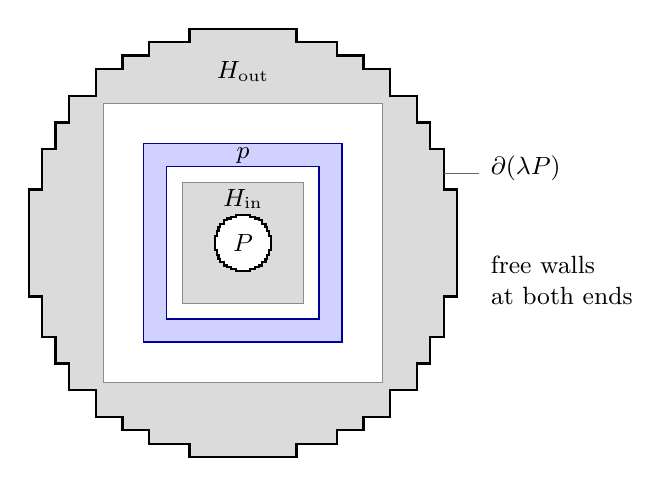
\begin{tikzpicture}[scale=.68, every node/.style={font=\small}]
 \def\wall{(4,0)--(4,1)--(3.75,1)--(3.75,1.75)
 --(3.5,1.75)--(3.5,2.25)--(3.25,2.25)--(3.25,2.75)
 --(2.75,2.75)--(2.75,3.25)--(2.25,3.25)--(2.25,3.5)
 --(1.75,3.5)--(1.75,3.75)--(1,3.75)--(1,4)
 --(-1,4)--(-1,3.75)--(-1.75,3.75)--(-1.75,3.5)
 --(-2.25,3.5)--(-2.25,3.25)--(-2.75,3.25)--(-2.75,2.75)
 --(-3.25,2.75)--(-3.25,2.25)--(-3.5,2.25)--(-3.5,1.75)
 --(-3.75,1.75)--(-3.75,1)--(-4,1)--(-4,-1)
 --(-3.75,-1)--(-3.75,-1.75)--(-3.5,-1.75)--(-3.5,-2.25)
 --(-3.25,-2.25)--(-3.25,-2.75)--(-2.75,-2.75)--(-2.75,-3.25)
 --(-2.25,-3.25)--(-2.25,-3.5)--(-1.75,-3.5)--(-1.75,-3.75)
 --(-1,-3.75)--(-1,-4)--(1,-4)--(1,-3.75)
 --(1.75,-3.75)--(1.75,-3.5)--(2.25,-3.5)--(2.25,-3.25)
 --(2.75,-3.25)--(2.75,-2.75)--(3.25,-2.75)--(3.25,-2.25)
 --(3.5,-2.25)--(3.5,-1.75)--(3.75,-1.75)--(3.75,-1)
 --(4,-1)--cycle}
 \fill[black!14] \wall;
 \fill[white] (-2.6,-2.6) rectangle (2.6,2.6);
 \fill[blue!18] (-1.85,-1.85) rectangle (1.85,1.85);
 \fill[white] (-1.42,-1.42) rectangle (1.42,1.42);
 \fill[black!14] (-1.125,-1.125) rectangle (1.125,1.125);
 \draw[black!45] (-2.6,-2.6) rectangle (2.6,2.6);
 \draw[blue!60!black] (-1.85,-1.85) rectangle (1.85,1.85);
 \draw[blue!60!black] (-1.42,-1.42) rectangle (1.42,1.42);
 \draw[black!45] (-1.125,-1.125) rectangle (1.125,1.125);
 \draw[thick] \wall;
 \begin{scope}[scale=.13]
  \fill[white] \wall;
  \draw[thick] \wall;
 \end{scope}
 \node at (0,0) {\(P\)};
 \node at (0,.82) {\(H_{\mathrm{in}}\)};
 \node at (0,1.64) {\(p\)};
 \node at (0,3.2) {\(H_{\mathrm{out}}\)};
 \node[anchor=west] at (4.45,1.4) {\(\partial(\lambda P)\)};
 \draw[black!60] (4.4,1.3)--(3.75,1.3);
 \node[anchor=west,align=left] at (4.45,-.7)
    {free walls\\at both ends};
\end{tikzpicture}

 \caption{A polygonal annulus with its full square guard \(p\) and the
 two possible end regions. The inner and outer walls are rectilinear
 approximations to circles; the square boundaries belong to the
 bands, not to the annular walls. Radial distances are compressed:
 the actual walls are \(P\) and \(\lambda P\), the guard is at scale
 \(\sqrt\lambda\), and either end is separated from it by a round
 annulus of logarithmic length
 \(\frac12\log\lambda-O(1)\). The two end regions are displayed
 together, but the pin estimate is applied to one end at a time.}
 \label{annuli:figure}
\end{figure}

Consider the centered, free height law \(\mu\) on this annulus, with
one common translation quotiented out. For a nonempty vertex set \(Q\),
write
\[
 [Q]=\{h_x=h_y\text{ for every }x,y\in Q\}.
\]
Thus \([Q]\) pins all differences within \(Q\), without pinning its
common height. For \(H=H_{\mathrm{in}}\) or \(H_{\mathrm{out}}\), set
\[
 \overline D(H,p)
   =\log\frac{\mu([H]\mid[p])}{\mu([H])}.
\]

\begin{proposition}[Separated flat pins]\label{annuli:flat-interaction}
Fix \(P\) as above. For either choice of \(H\), the interaction
\(\overline D(H,p)\) is nonnegative and
\begin{equation}
 \limsup_{\mathrm{mesh}\to0}\overline D(H,p)
 \quad\text{can be made arbitrarily small by taking \(\lambda\) large.}
 \tag{7}\label{eq:source-7}
\end{equation}
The mesh limit is taken at each fixed polygonal geometry.
\end{proposition}

The proof of Proposition~\ref{annuli:flat-interaction} first estimates
the continuum interaction with one confining
box average. It then weakens that confinement and passes from absolute
pins to flat pins. The constant mode is retained throughout.

\subsection{The continuum estimate with confinement}

Choose a dyadic box inside \(p\) whose side lengths are fixed positive
multiples of \(\sqrt\lambda\), and let \(B_0\) be its probability
average. Sum all common height translations and add the penalty
\(\gamma(B_0h)^2/2\), where \(\gamma>0\). Let \(D_\gamma(H,p)\)
be the interaction of the absolute events \(h_H=0\) and \(h_p=0\)
under this confined law.

Start with \(\gamma=1\). By Theorem~\ref{heights:pin-input},
\(D_1\) converges to the Gaussian
interaction for
\[
 \mathcal T(u)=a^{-1}\int_{A_\lambda}|\nabla u|^2+(B_0u)^2.
\]
Write \(\|u\|_{\mathcal T}^2=\mathcal T(u)\).
As in Equation~\eqref{eq:source-1}, let
\[
 V_Q=\{u\in H^1(A_\lambda):u=0\text{ on }Q\}^{\perp_{\mathcal T}},
 \qquad C=\Pi_H|_{V_p}.
\]
We claim that \(\|C\|_{\mathrm{HS}}\to0\) as \(\lambda\to\infty\).

Between \(p\) and \(H\) there is a full round annulus which is a
conformal cylinder
\begin{equation}\label{annuli:cylinder}
 [0,T]\times\bigl(\R/(2\pi\Z)\bigr),\qquad
 T=\tfrac12\log\lambda-O(1).
\end{equation}
The end \(s=0\) faces \(p\). For the inner end, for example, one may
take radii \(8\) and \(\sqrt\lambda/2\), with the logarithmic coordinate
reversed. For the outer end one may take radii \(4\sqrt\lambda\) and
\(\lambda/8\). Enlarging the lower bound on \(\lambda\) makes both
choices available, with fixed clearances from the bands.

For \(f\in V_p\), the trace at \(s=0\) satisfies
\begin{equation}\label{annuli:trace}
 \|f|_{s=0}\|_{H^{1/2}(\mathbb S^1)}
       \le C_0\|f\|_{\mathcal T},
\end{equation}
with \(C_0\) independent of large \(\lambda\). Indeed, after scaling
lengths by \(\sqrt\lambda\), this circle, the guard, and the observation
box lie in a fixed connected annular region. Poincare's inequality
with the box mean controls the \(H^1\) norm there, including constants;
the trace theorem then gives Equation~\eqref{annuli:trace}.
On the side of this circle containing \(H\), the function \(f\)
minimizes the gradient energy with its given trace and free walls.
There is no observation term on that side.

Let \(A\) map a trace at \(s=0\) to the restriction to \(H\) of this
energy minimizer, with the target norm equal to the least
\(\mathcal T\)-norm of an extension of that restriction to the whole
annulus. This target is naturally identified with \(V_H\).
We estimate \(A\) on a normalized Fourier basis of \(H^{1/2}(\mathbb S^1)\).
For the constant trace, the minimizer on the \(H\)-side is constant.
An extension of its \(H\)-data can be chosen constant beyond \(s=T\),
linear across the cylinder, and zero before \(s=0\). It vanishes on
the observation box and has energy \(O(T^{-1})\). Thus the norm of
the image of the constant mode is \(O(T^{-1/2})\).

For a sine or cosine mode of frequency \(j\ge1\), normalization in
\(H^{1/2}\) makes its amplitude \(O((1+j)^{-1/2})\).
The Neumann minimum at \(s=T\), on the cylinder alone, is a lower
bound for the actual minimum. The Dirichlet-zero minimum at \(s=T\),
extended by zero beyond that circle, is an admissible upper trial.
The solutions of \(u''=j^2u\) give, respectively, the factors
\(\tanh(jT)\) and \(\coth(jT)\) in their energies. Their difference
is therefore \(O(e^{-2jT})\). Orthogonality of the actual minimizer
to zero-trace variations shows that the difference between it and
the upper trial has gradient norm \(O(e^{-jT})\). This difference
has zero trace at \(s=0\), so it extends by zero toward \(p\), pays no
observation penalty, and has, up to sign, the required restriction
on \(H\). Consequently
\[
 \|A\|_{\mathrm{HS}}^2
       \le \frac{C_1}{T}+C_1\sum_{j\ge1}e^{-2jT}
       \longrightarrow0.
\]
All extensions are in \(H^1\): across each interior circle their
traces agree. Composing \(A\) with the uniformly bounded trace map
in Equation~\eqref{annuli:trace} proves the claim for \(C\).
The determinant in Equation~\eqref{eq:source-1} now tends to one,
since \(\|C\|\le\|C\|_{\mathrm{HS}}\to0\). We have proved
\begin{equation}\label{annuli:unit-confinement}
 \lim_{\lambda\to\infty}\lim_{\mathrm{mesh}\to0}D_1(H,p)=0.
\end{equation}

\subsection{From absolute pins to flat pins}

We next establish Equation~\eqref{annuli:unit-confinement} with any
fixed \(\gamma>0\) in place of \(1\). Consider the four partition
functions defining the absolute-pin interaction. When \(p\) is
pinned, \(B_0h=0\), so changing \(\gamma\) has no effect. With neither
region pinned, the ratio of partition functions at precisions
\(\gamma\) and \(1\) tends to \(\gamma^{-1/2}\). This follows from
Theorem~\ref{heights:mixed-input}: the fractional mean becomes uniform and
independent of the mean-free field, and the translation sums of the
Gaussian penalties are bounded periodic functions.

With \(H\) alone pinned, let \(x=x(\lambda)\) be the variance of \(B_0\)
in the massless continuum Gaussian law with that pin. Applying the
hard-pin height limit in Theorem~\ref{heights:mixed-input} to the two bounded weights
\(\exp(-\gamma(B_0h)^2/2)\) and \(\exp(-(B_0h)^2/2)\) gives the ratio
\[
 \left(\frac{1+x}{1+\gamma x}\right)^{1/2}.
\]
Moreover \(x\to\infty\). To see this from the variational formula for
the variance, take a function equal to one on the \(p\)-side, zero
on the \(H\)-side, and linear across the cylinder
in Equation~\eqref{annuli:cylinder}. Its box average is one and
its gradient energy is \(O(T^{-1})\), so \(x\ge cT\).
Combining the four partition functions yields, at fixed geometry,
\begin{equation}\label{annuli:change-confinement}
 D_\gamma-D_1\longrightarrow
       \frac12\log\frac{1+\gamma x}{\gamma(1+x)}.
\end{equation}
The right side tends to zero as \(\lambda\to\infty\). The absolute-pin
interaction thus tends to zero for every fixed positive \(\gamma\).

It remains to compare these absolute pins with the desired flat
events. In a centered confined law, the logarithmic interaction of
two centered quadratic penalties increases when either precision
increases. In fact, if the first precision changes by \(tQ\),
differentiating the four log partition functions gives
\[
 \frac12\Tr Q\bigl(\Cov_{\text{first penalty}}
                    -\Cov_{\text{both penalties}}\bigr)\ge0
\]
by centered covariance comparison. Taking equality limits proves
the same assertion for nested centered constraints. Absolute zero
pins are obtained from flat pins by also pinning one reference
height in each set after the within-set constraints are imposed.
Hence the interaction of \([H]\) and \([p]\)
in the confined law is between zero and \(D_\gamma(H,p)\).

Finally, project the confined law onto common-translation orbits.
If \(t=B_0h\) in any representative, the orbit receives the factor
\[
 w_\gamma(t)=\sum_{k\in\Z}
       \exp\{-\tfrac{\gamma}{2}(t+2\pi k)^2\}.
\]
Poisson summation gives the uniform estimate
\[
 \sup_t\left|\sqrt{2\pi\gamma}\,w_\gamma(t)-1\right|
 \le 2\sum_{j\ge1}e^{-j^2/(2\gamma)}
       =:\delta_\gamma\longrightarrow0
       \qquad(\gamma\downarrow0).
\]
For \(\gamma\) sufficiently small that \(\delta_\gamma<1\), the
normalized projected density relative to the free
orbit law is between
\((1-\delta_\gamma)/(1+\delta_\gamma)\) and its reciprocal.
This multiplicative estimate applies to the individual pin events
and their intersection, however small their probabilities. Their
log interactions differ by \(O(\delta_\gamma)\), uniformly in the
mesh and the annulus.

Given a tolerance, first choose \(\gamma>0\) so that this error is
small. Then choose \(\lambda\) large so that the limiting absolute-pin
interaction is small, and finally take the mesh limit at that
fixed geometry. This proves Equation~\eqref{eq:source-7}.
Nonnegativity in the free law follows either from centered
precision comparison directly or by sending \(\gamma\) to zero
at each fixed finite graph.
\qed
